\documentclass{article}
\usepackage{amsmath}
\usepackage{amssymb}
\usepackage{graphicx}
\usepackage{hyperref}
\usepackage[version=4]{mhchem}

\title{Example 5}
\date{}

\begin{document}
\maketitle

As shown in the figure below, in \(\triangle A B C, A B>A C . A D\) is the angle bisector of \(\angle A\). Show that \(A B-A C>E B-E C\).

Solution:
Take \(F\) on \(A B\) so that \(A F=A C\).\\
\centering
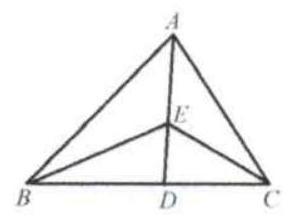
\includegraphics[width=\textwidth]{images/problem_image_1.jpg}\\
\(A B-A C=A B-A F=B F\).\\
Since \(A D\) is the angle bisector of \(\angle A, A E\) is the angle bisector of \(\angle A\), and \(A F=A C, A E=A E\). So we have \(\triangle A E F\) \(\cong \triangle A E C\). Therefore \(E F=E C\).

By triangle inequality theorem, in \(\triangle B E F, B F>E B-E F=\)\\
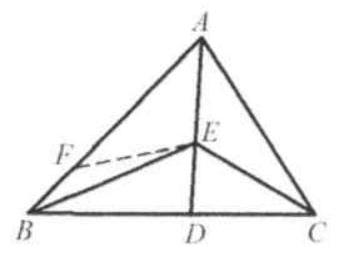
\includegraphics[width=\textwidth]{images/reasoning_image_1.jpg} \(E B-E C\), or \(A B-A C>E B-E C\).


\end{document}
